\documentclass[a4paper , 12pt]{article}
\usepackage{enumerate}
\usepackage{graphicx}
\usepackage{amsmath}
\usepackage{pdfpages}
\usepackage{graphicx}
\usepackage{epstopdf}
\usepackage{caption}
\usepackage{subcaption}
\usepackage{amsmath}
\usepackage{color}
\usepackage{listings} %to insert matlab code
\lstset{language=C,commentstyle=\color{blue}} 
\usepackage{nomencl}
\makenomenclature

% Title Page
\addtolength{\oddsidemargin}{-1in}
	\addtolength{\evensidemargin}{-1in}
	\addtolength{\textwidth}{1.4in}

	\addtolength{\topmargin}{-1.5in}
	\addtolength{\textheight}{1.75in}
\title{ ED 3110 : Product Design Lab. 2\\
   {\small {\large I-Glide: Self-balancing Personal Transporter}} }
\author{ Rohan Chavan - ED11B010\\
		Piyush Jadav - ED11B018\\
		Dhruvesh Patel - ED11B026\\
		Shambhuraj Sawant - ED11B034
		}


\begin{document}
\maketitle

\begin{abstract}
\textbf{}
\end{abstract}\newpage

\tableofcontents\newpage
\newpage
\section{Problem Statement}
To develop a product that addresses the short distance transportation (2-7 km) issues of people across age groups while keeping the product compact, portable and safe.
 
\subsection{Motivation}
Around $ 85\% $ of students in institute either took public transport or cycled to reach their desired destination. But this model had its deficit. Students complained about parking issues and bike getting stolen or damaged. \\
\newline
When we interacted with the older age group they complained about safety and parking issues issues and an absence of transport option that could directly reach their doorstep. Other issues also included significant waiting times and overcrowding in public transportation systems. \\ 
\newline
We wanted a solution that could address all of these issues. This required the final product to be portable, compact and easy to use on daily basis.
\newline

\subsection{Market}
The next step was to study the market that could be targeted. There is a lot of scope for a product like this, if tweaked as per the needs as the range would further widened
\begin{enumerate}
\item \textbf{Students and middle-aged group:} Our primary target, here the product could eliminate issues mentioned above.
\item \textbf{Mall, airport and hotel staff:} The product could be modified to provide safe, stable transport with an option to carry luggage.
\item \textbf{Movement of operators in multi-bay plants:} This would reduce waiting times and increase plant efficiency.
\end{enumerate}

\subsection{Existing products}
Products in the market targetting these problems include Scarpar, Segway and Electric skateboards among others. But every option here had their disadvantages such as expensive, heavy, availability etc

\newpage
\section{Our Ideation}

\begin{figure}[ha!]
\centering
   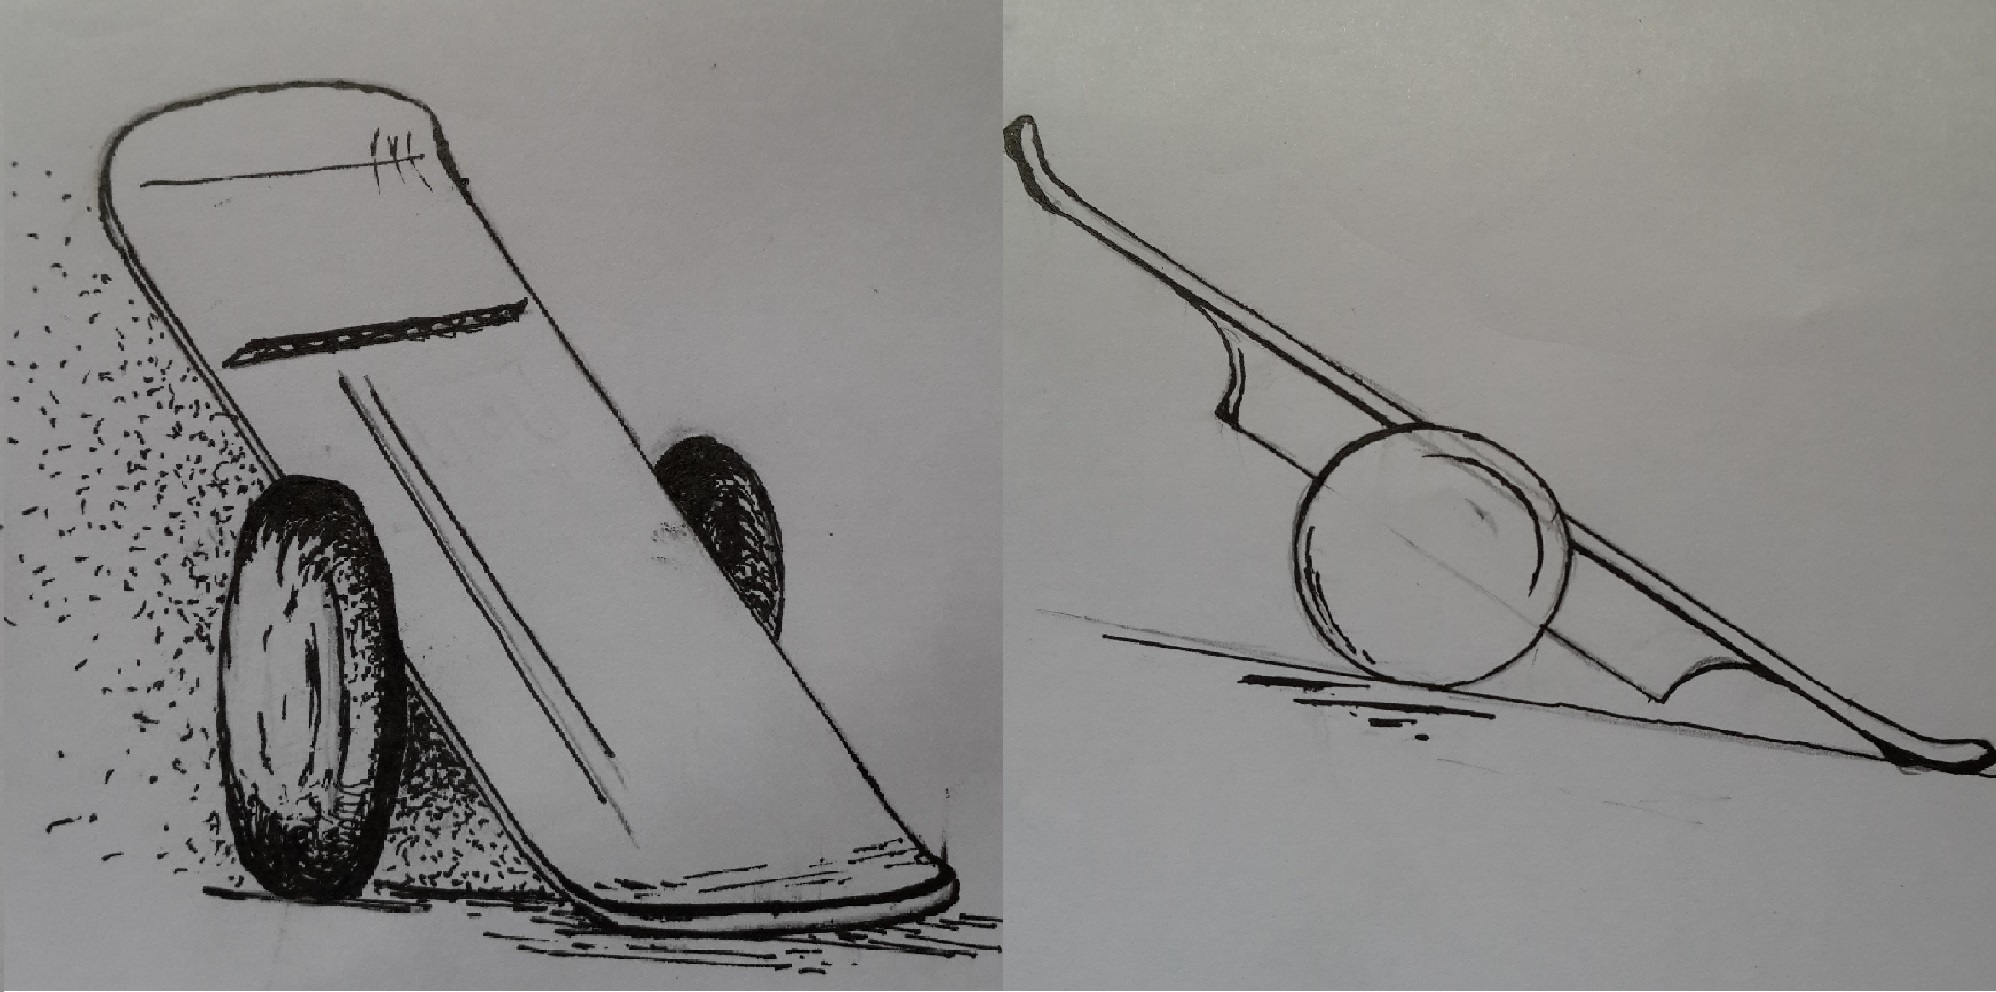
\includegraphics[width=120mm]{first_concept}
        \caption{Initial layout}
        \end{figure}
        
\subsection{What is it?}
\begin{itemize}
\item A self balancing 2 wheeled transporter
\item Focusing on basic control algorithm for safe propulsion 
\item Compactness and portability to some extent.
\item Provided with straps to carry around.
\item Design can be extended further to include variants of the same to meet different market needs and safety requirements. 

\end{itemize}
\newpage
\section{Technical feasibility }
The existing literature of \textit{mobile inverted pendulum} was studied thoroughly ([1],[2]). It was concluded from this study that though the dynamics of the system is nonlinear, linear approximation works very well in a sufficiently large range. \\ 

The dynamics of the system was modelled using Newton's laws and linearised to arrive at the following state space model.\\
\renewcommand{\nomname}{{\normalsize Here,}}
\nomenclature{Mb}{$\rightarrow$ Mass of the pendulum}
\nomenclature{Mw}{$\rightarrow$ Mass of the wheels}
\nomenclature{Ke,Km}{$\rightarrow$ Motor constants}
\nomenclature{R}{$\rightarrow$ Motor armature resistance}
\nomenclature{Rw}{$\rightarrow$ Radius of wheels}
\nomenclature{L}{$\rightarrow$ Height of the pendulum (person)}
\nomenclature{Jb}{$\rightarrow$ Moment of inertia of the person about their center of mass}
\nomenclature{Jw}{$\rightarrow$ Moment of inertia of wheels}
\nomenclature{g}{$\rightarrow$ Acceleration due to gravity}
\nomenclature{V(t)}{$\rightarrow$ Control voltage}
\textbf{States:}
$$
\textbf{x}=\left(
\begin{array}{c}
y(t)\\
y'(t)\\
\theta(t)\\
\theta'(t)
\end{array}
\right)
$$

\textbf{Dynamics matrix:}
$$
\textbf{A}=\left(
\begin{array}{cccc}
 0 & 1 & 0 & 0 \\
 0 & \frac{2 \text{Ke} \text{Km} \left(-\text{Mb} L^2+\text{Mb}
   \text{Rw} L-\text{Jb}\right)}{R \left(2 \text{Mb}
   \left(\frac{\text{Jw}}{\text{Rw}^2}+\text{Mw}\right)
   L^2+\text{Jb} \left(\frac{2 \text{Jw}}{\text{Rw}^2}+\text{Mb}+2
   \text{Mw}\right)\right) \text{Rw}^2} & \frac{g L^2 \text{Mb}}{2
   \text{Mb} \left(\frac{\text{Jw}}{\text{Rw}^2}+\text{Mw}\right)
   L^2+\text{Jb} \left(\frac{2 \text{Jw}}{\text{Rw}^2}+\text{Mb}+2
   \text{Mw}\right)} & 0 \\
 0 & 0 & 0 & 1 \\
 0 & \frac{2 \text{Ke} \text{Km} \left(\left(\frac{2
   \text{Jw}}{\text{Rw}^2}+\text{Mb}+2 \text{Mw}\right)
   \text{Rw}-L \text{Mb}\right)}{R \left(2 \text{Mb}
   \left(\frac{\text{Jw}}{\text{Rw}^2}+\text{Mw}\right)
   L^2+\text{Jb} \left(\frac{2 \text{Jw}}{\text{Rw}^2}+\text{Mb}+2
   \text{Mw}\right)\right) \text{Rw}^2} & \frac{g L \text{Mb}
   \left(\frac{2 \text{Jw}}{\text{Rw}^2}+\text{Mb}+2
   \text{Mw}\right)}{2 \text{Mb}
   \left(\frac{\text{Jw}}{\text{Rw}^2}+\text{Mw}\right)
   L^2+\text{Jb} \left(\frac{2 \text{Jw}}{\text{Rw}^2}+\text{Mb}+2
   \text{Mw}\right)} & 0 \\
\end{array}
\right)
$$
\\
\textbf{Input coupling matrix:}
% B matrix
$$
\textbf{B}=\left(
\begin{array}{c}
 0 \\
 \frac{2 \text{Km} \left(\text{Mb} L^2-\text{Mb} \text{Rw}
   L+\text{Jb}\right)}{R \left(2 \text{Mb}
   \left(\frac{\text{Jw}}{\text{Rw}^2}+\text{Mw}\right)
   L^2+\text{Jb} \left(\frac{2 \text{Jw}}{\text{Rw}^2}+\text{Mb}+2
   \text{Mw}\right)\right) \text{Rw}} \\
 0 \\
 \frac{2 \text{Km} \left(L \text{Mb}-\left(\frac{2
   \text{Jw}}{\text{Rw}^2}+\text{Mb}+2 \text{Mw}\right)
   \text{Rw}\right)}{R \left(2 \text{Mb}
   \left(\frac{\text{Jw}}{\text{Rw}^2}+\text{Mw}\right)
   L^2+\text{Jb} \left(\frac{2 \text{Jw}}{\text{Rw}^2}+\text{Mb}+2
   \text{Mw}\right)\right) \text{Rw}} \\
\end{array}
\right)
$$
\\
\textbf{Input:}
$$
u= V(t)
$$
\\ State space equation:
$$
\textbf{x}'(t)=\textbf{A}\textbf{x}(t) + \textbf{B}u(t)
$$

\printnomenclature

\newpage
\section{Manufacturing}
\subsection{layout}
\begin{figure}[ha!]
\centering
   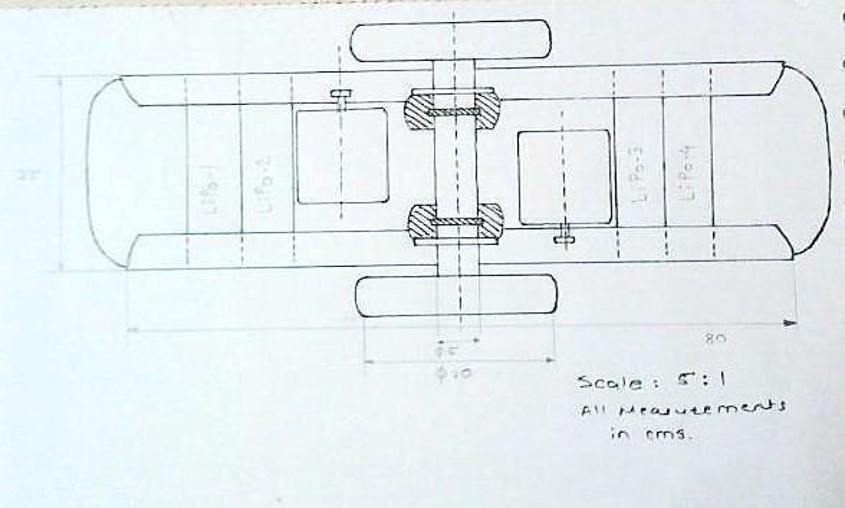
\includegraphics[width=120mm]{layout_1}
        \caption{layout of components on the board}
        \end{figure}
        
      
\subsection{Design Parameters}
\begin{itemize}
\item To maintain a low centre of gravity all the components were placed on the bottom
\item Components should not hit ground as than balancing and therefore controlling would be difficult plus damages to product
\item The centre of gravity could not lowered to an extent that there would be difficulties placing the components below. 
\end{itemize}
\begin{figure}[ha!]  
\centering
   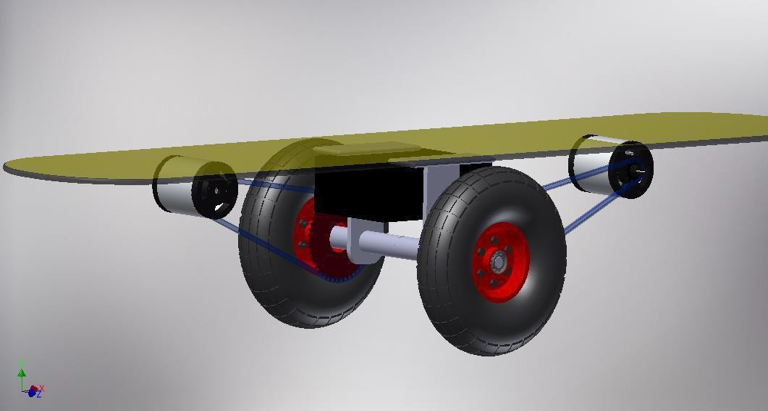
\includegraphics[width=120mm]{cad_1}
        \caption{Our final CAD model}
        \end{figure}
        
\subsection{Initial assembly}
The assembly consisted of three major parts - \textit{Motor and wheel, axle and platform}. The idea was to check for part availability in the market and than start with actual manufacturing. 
\begin{enumerate}
\item Wheels used here (\textit{fig. 4}) are electric scooter wheels
\item A safety factor of 1.75 was considered while designing the axles
\item We faced a lot of issues with these mounts and hence we changed them with bushes
\end{enumerate}
\begin{figure}[ha!]

\centering
   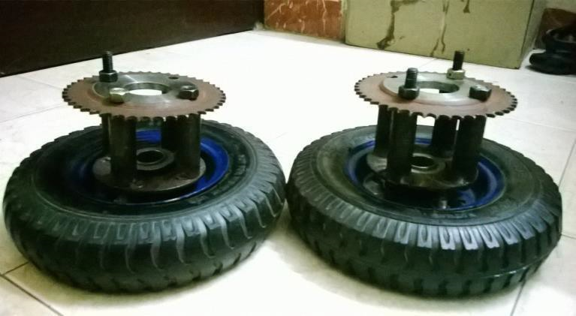
\includegraphics[width=120mm]{wheel_des_1}
        \caption{Wheel assembly with sprockets}
        \end{figure}
 
\begin{figure}[ha!]

\centering
   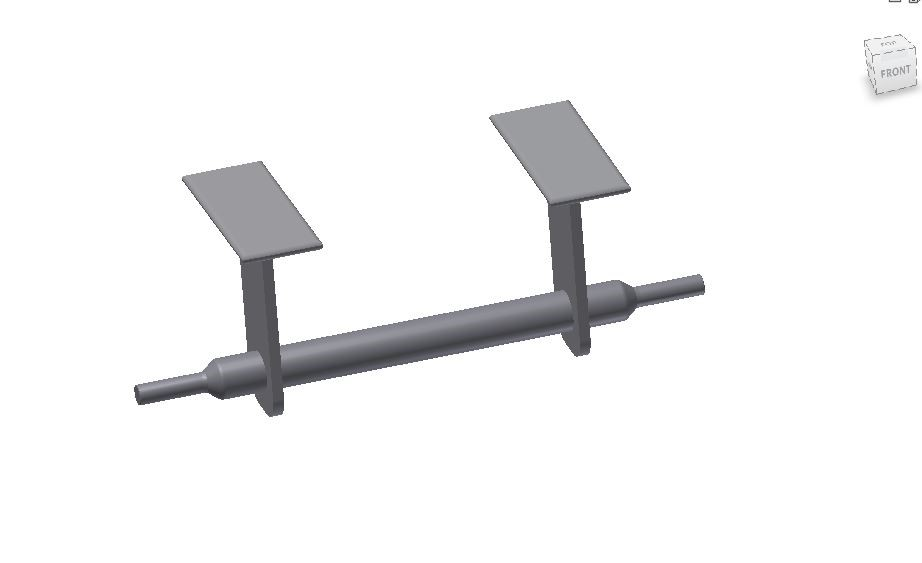
\includegraphics[width=120mm]{axle_1}
        \caption{Axle CAD model}
        \end{figure}  
        
\begin{figure}[ha!]

\centering
   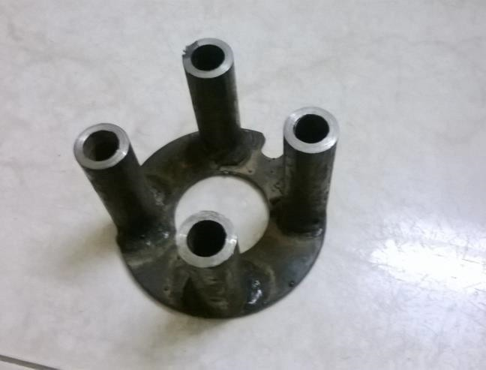
\includegraphics[width=120mm]{sprocket_des_1}
        \caption{Wheel-sprocket mounts}
        \end{figure} 
        
        
\begin{table}[h] 
\caption{Dimensions of components} 
\centering
\begin{tabular}{c c c c}
\hline\hline
Parts & Symbol	& Dimensions &	Weight \\
\hline
Wheels	& $D$	& 25cm	& 2 kg\\
Deck	& $L$ x W x H	& 80cm x 35cm x 2cm	& 2.25 kg\\
Motors	& $d1$	& 10cm	& 4 kg\\
Battery	& $L1 X W1$	& 15cm X 6cm	& 2.2 kg\\
sprocket diameter	& $D2$	& 12.5cm	\\
pitch of the chain	&$ p$	& 8mm	& 0.7 kg\\
chain length	& $(30)*p$	& 24cm	& NA\\
distance between tires	& $a$	& 40cm	& 4.7 kg (axle+sprocket+wheel)\\
\hline
 \end{tabular}
 \end{table}
 
Also it was seen that, the weight distribution is uniform
\pagebreak

\newpage

\section{Electronics}
Electronics part of I-glide consists of basic modules:
\begin{enumerate}
\item	Sensing module:
It consists of following parts:
Razor IMU (SEN-10736 RoHS), FTDI Basic Breakout – 3.3V (DEV-09873 RoHS)
\item	Actuator module:
It consists of following parts: 
2X 2500 RPM motor, 2X 12V Lead-acid batteries, 2X DC motor drivers
\item	Processing module:
It consists of following parts:
 Arduino UNO.
\item	Electrical assembly:
It consists of general electrical components like
10, 15, 20A fuse, 10V and 24V switches, LEDs, Prototype board.
\end{enumerate}

\textbf{Circuit Schematic:}
\begin{figure}[ha!]

\centering
   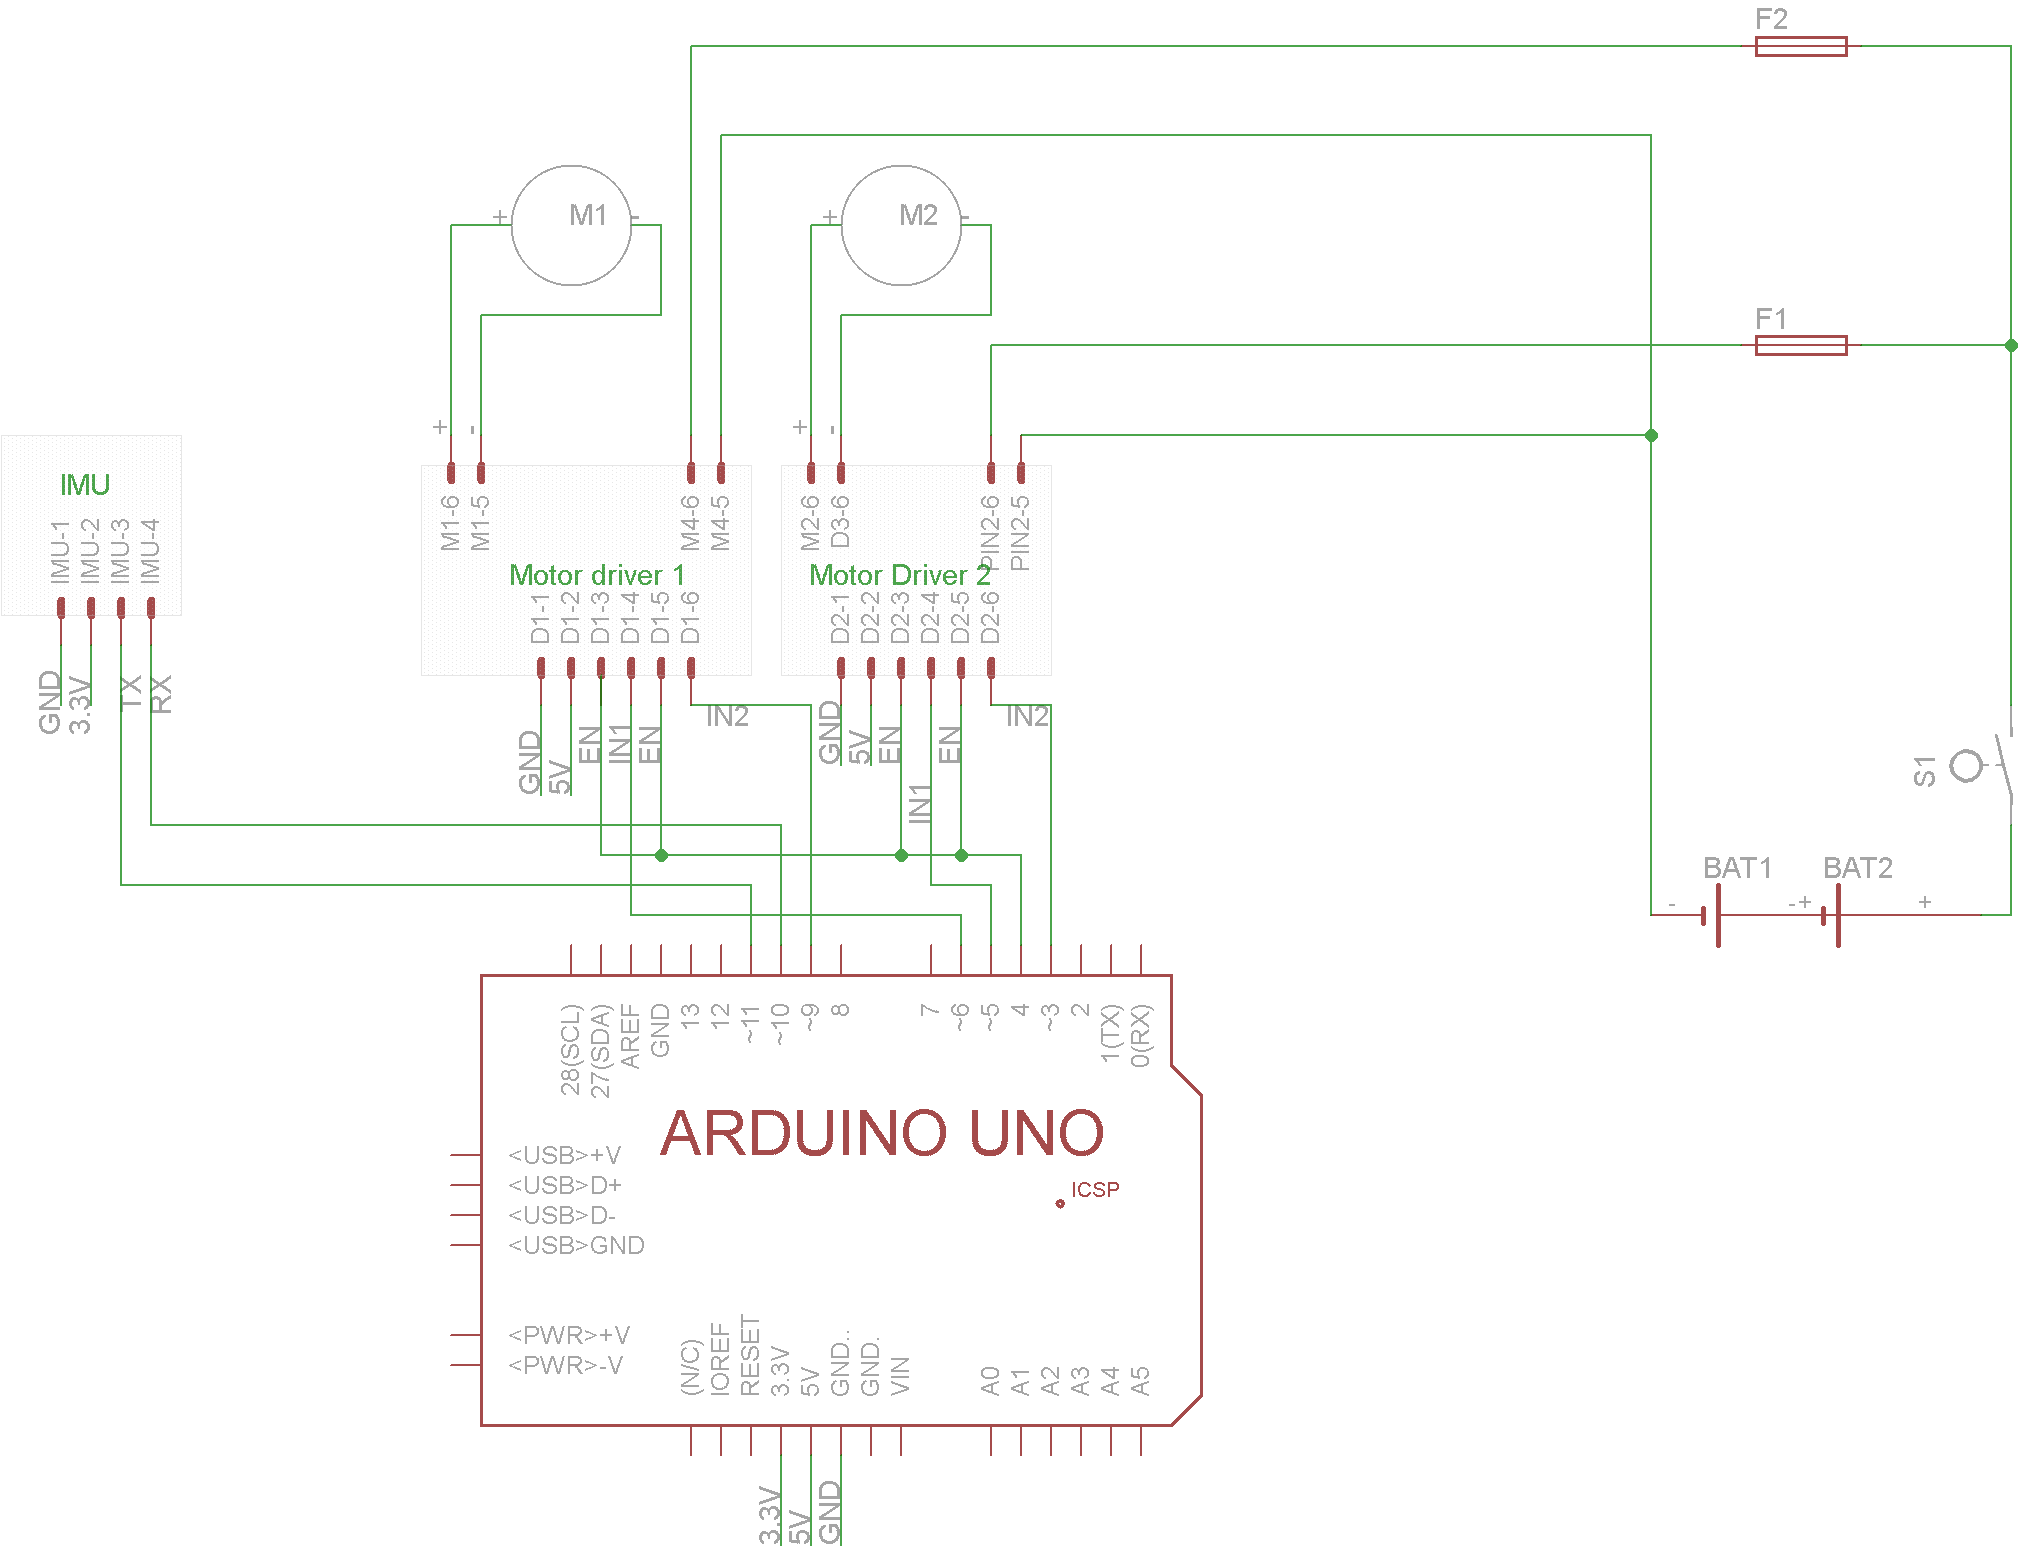
\includegraphics[width=120mm]{circuit1}
        \caption{Circuit}
        \end{figure}

\pagebreak
\subsection{Code and Algorithm}
For the first implementation PID controller for pitch angle was used. The code is as follows:

	\begin{lstlisting}[frame=single]
	
	#include <SoftwareSerial.h> 
	/* To support serial communication with 
	2 devices simultaneously*/

	SoftwareSerial mySerial(12, 11); 
	/* RX, TX  Set the softSerial port */
	
	/*working variables of the pid*/
	unsigned long lastTime=0; 
	double Input=0, Output=0, Setpoint=0;
	double ITerm=0, lastInput=0;
	double kp, ki, kd,KP=0.005,KI=0,KD=0; 
	int pwm=0;
	const double slope=10.625; /* to scale the Output
	 in Voltage to appropriate PWM signal*/
	const int DirPin=4;
	const int M1pwmPin=3,M2pwmPin=9;
	int SampleTime=250; //.250 sec
	
	
	  
	void SetTunings(double Kp, double Ki, double Kd) 
	// Function to find gains for the discrete system
	{
	  double SampleTimeInSec = ((double)SampleTime)/1000;
	   kp = Kp;
	   ki = Ki*SampleTimeInSec;
	   kd = Kd/SampleTimeInSec;
	}
	
	 //Function to read the pitch angle value from IMU 
	double ReadPitch() 
	{
	 mySerial.print("#f");
	  while(mySerial.available()<12){};
	  
	   byte yaw[4];
	   byte pitch[4];
	   byte roll[4]; 
	   float y,p,r;
	   int i;
	   for(i=0;i<=3;i++)
	   {
	     yaw[i]=mySerial.read();
	     
	   }
	    for(int i=0;i<=3;i++)
	   {
	     pitch[i]=mySerial.read();
	   }
	    for(int i=0;i<=3;i++)
	   {
	     roll[i]=mySerial.read();
	   }
	  y=*(float *)&yaw;
	  p=*(float *)&pitch;
	  r=*(float *)&roll;
	 return(r);
	  
	}
	
	
	
	
	
	void setup() // Main Setup
	{
	   // Open serial communications and wait for port to open:
	  Serial.begin(9600);
	
	  // set the data rate for the SoftwareSerial port
	  mySerial.begin(9600);
	  pinMode(DirPin,OUTPUT); //Declare digital output
	}
	
	void loop() // Main loop
	{
	  double error;
	  Input= ReadPitch();
	  error= Setpoint - Input;
	 
	  while(error<=-10||error>=10) // Loop for soft start
	  { Input= ReadPitch();
	  error= Setpoint - Input;
	  }
	  
	 
	  SetTunings(KP,KI,KD);
	  lastTime=0;
	  pwm=0;
	 
	  while(1) //Main control loop
	  {
	  Input= ReadPitch();
	  error= Setpoint - Input;
	   
	  unsigned long now = millis(); // present timestamp
	  double timeChange = (double)(now - lastTime); // timechange
	  
	  if(timeChange>=SampleTime)
	  {
	    /*Compute all the working error variables*/
	   /*do only for pitch*/
	   ITerm += (ki * error);
	   double dInput = (Input - lastInput);
	  
	   /*Compute PID Output*/
	   Output = kp * error + ITerm - kd * dInput;
	  
	   /*Remember some variables for next time*/
	   lastInput = Input;
	   lastTime = now;
	  }
	  
	  /* Convert the Output into a signal which 
	  can be given to pwm */
	 if(Output>=0)
	{
	  pwm= int(slope*(Output));
	  analogWrite(M1pwmPin,pwm);
	  analogWrite(M2pwmPin,pwm);
	  digitalWrite(DirPin,HIGH);
	} 
	else
	{
	  pwm= int(slope*(-Output));
	  analogWrite(M1pwmPin,pwm);
	  analogWrite(M2pwmPin,pwm);
	  digitalWrite(DirPin,LOW);
	}
	  
	  if(pwm>100) // safety cutoff
	  {
	    break;
	  }
	  
	  }
	}
	\end{lstlisting} 
The filter and communication code on the controller on the IMU is quite complicated and hence given in Appendix-1 for the sake of completeness. 

\subsection{Problems faced}
\begin{enumerate}
\item	Serial communication problem: 
Razor IMU firmware was designed to give continuous streaming output, while arduino couldn’t handle this continuous stream. For this purpose, we needed to change the firmware a bit and write a separate module for communication. Finally everything synced together!
\item	Connectors:
This is the usual problem of any circuit, connection breaking in between or loose connection. To solve this, we used sealing gun.
\item	Motor Driver:
This problem was caused because of high initial current requirement of dc motor. Even after putting fuse, we lost 4 of our working motor drivers. We couldn’t fix this problem. For this purpose, total of 4 types of drivers were tried, but none of them worked successfully. The best way to overcome this problem would be to build our own motor driver based on H-bridge circuit.

\end{enumerate}

\newpage
\section{Appendix}
\begin{enumerate}[(A)]
\item
\textbf{Mathematica code to obtain closed loop system}
	\begin{figure}[!ht]
		\centering
		  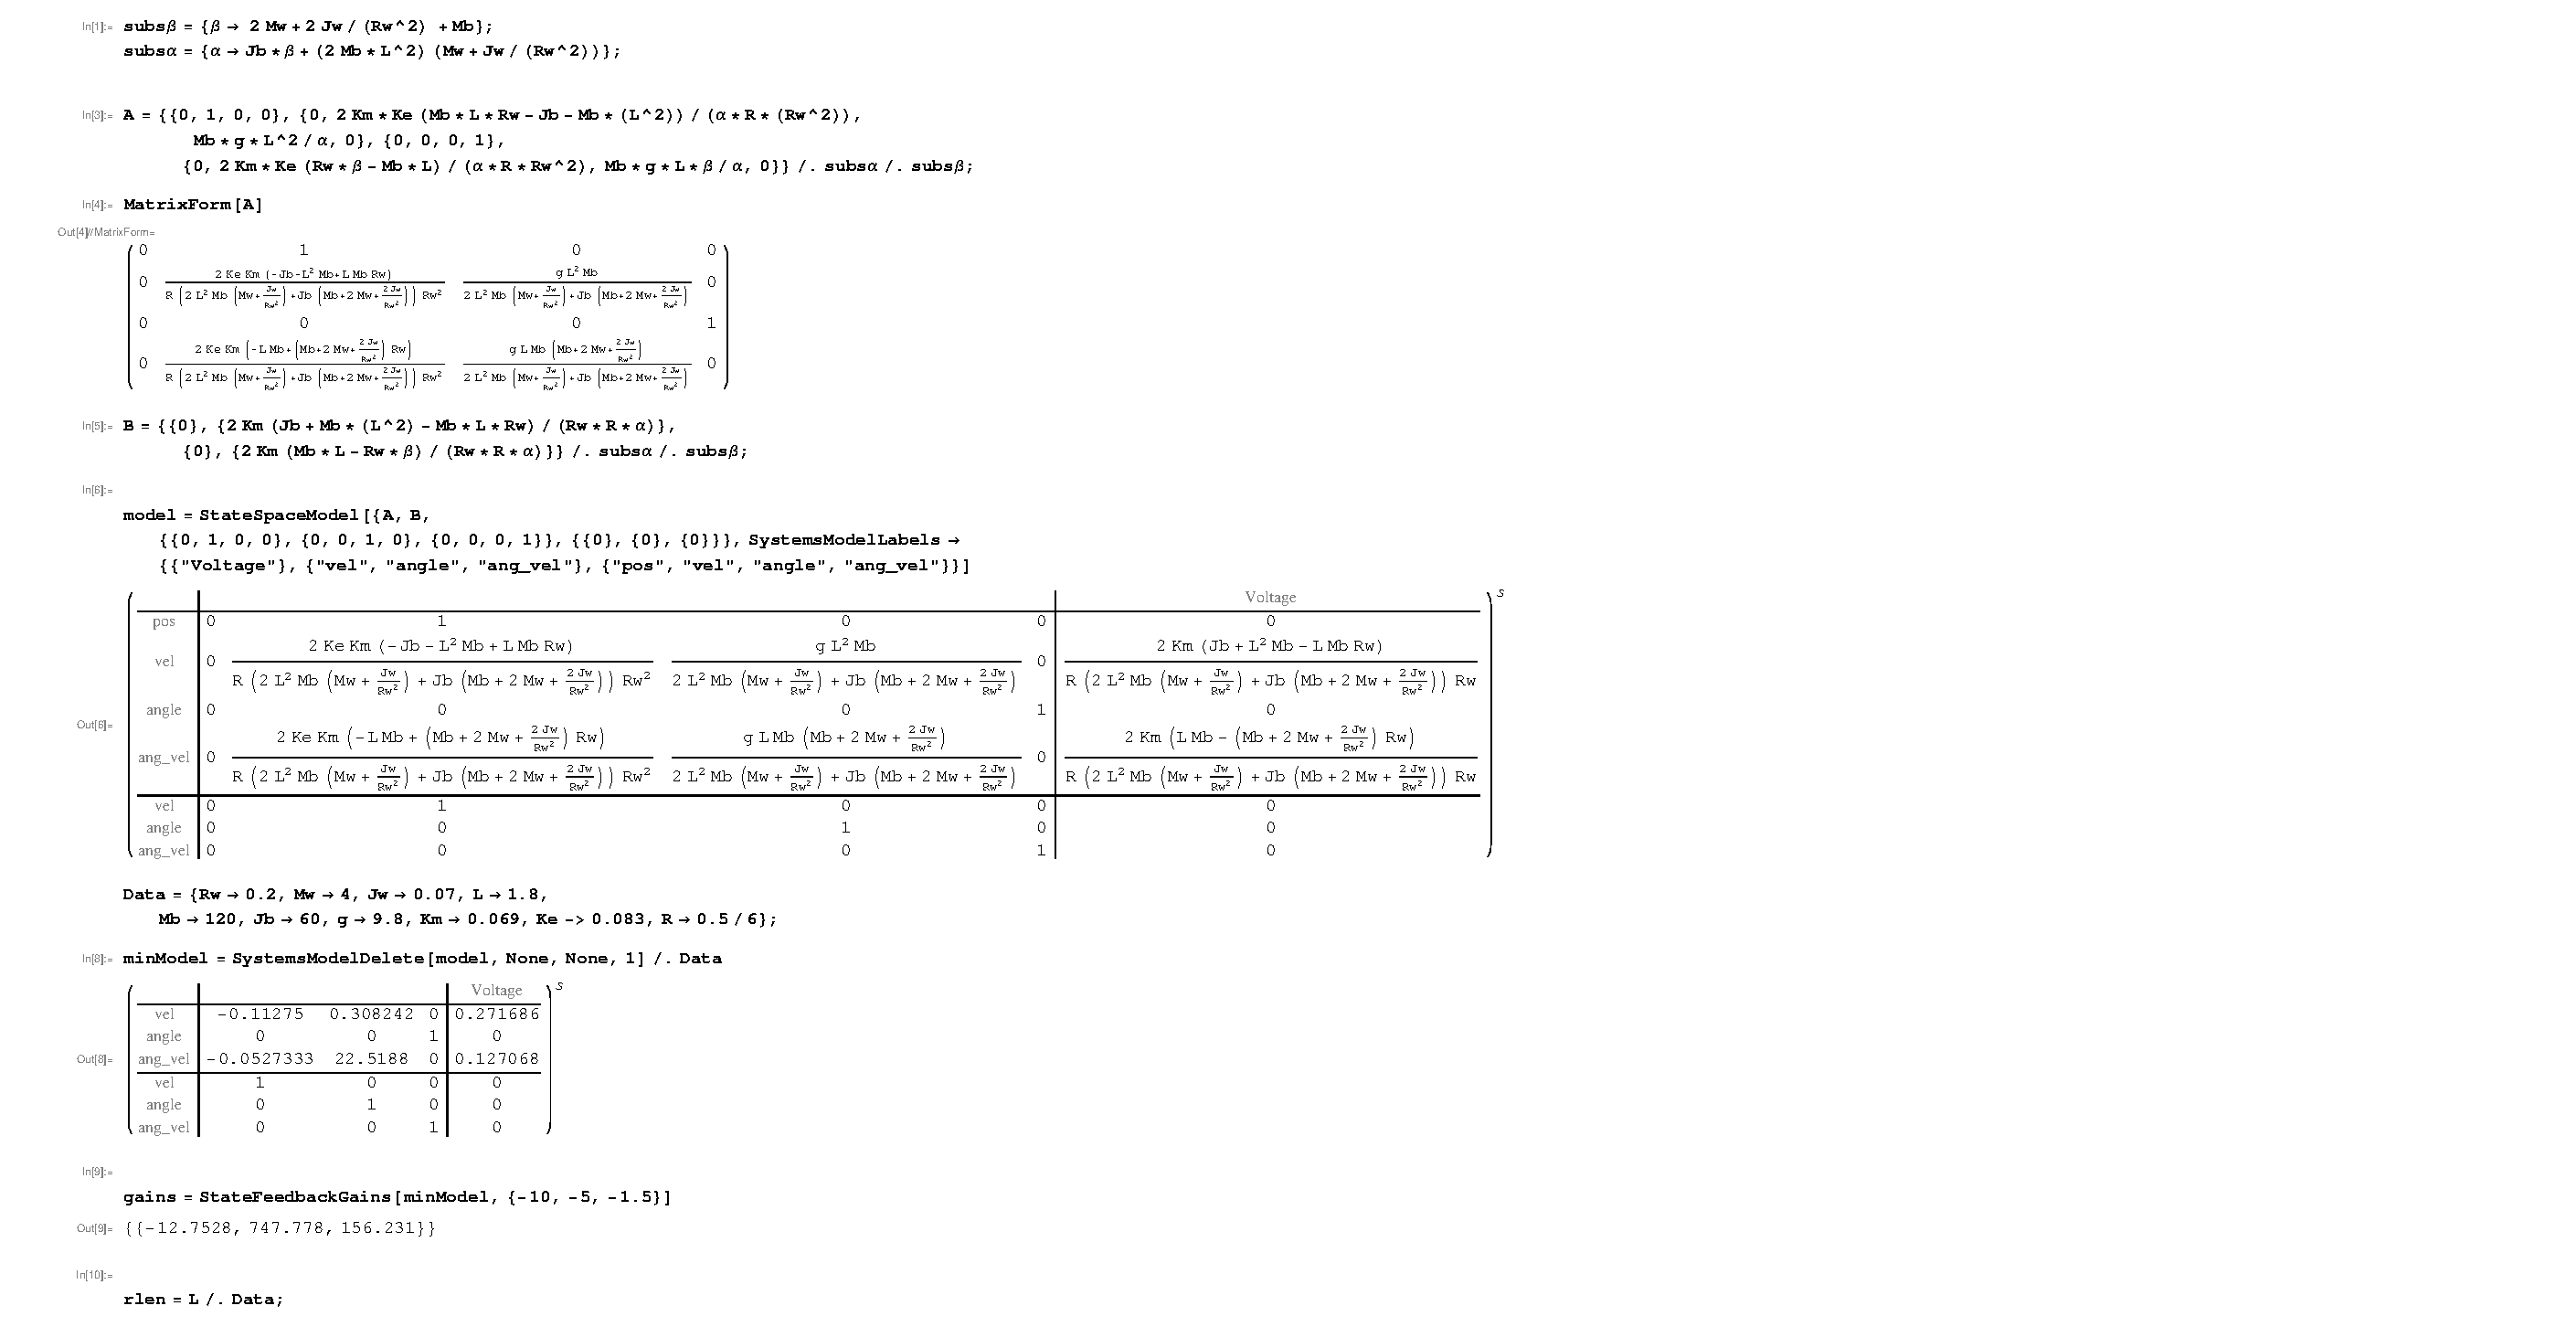
\includegraphics[width=1.8 \linewidth]{code1.eps}
		  \caption{Code to obtain closed loop system}
		  \label{fig:6.1}
	\end{figure}
	\newpage
\textbf{ Code added for simulation and visualization}
\begin{figure}[!ht]
		\centering
		  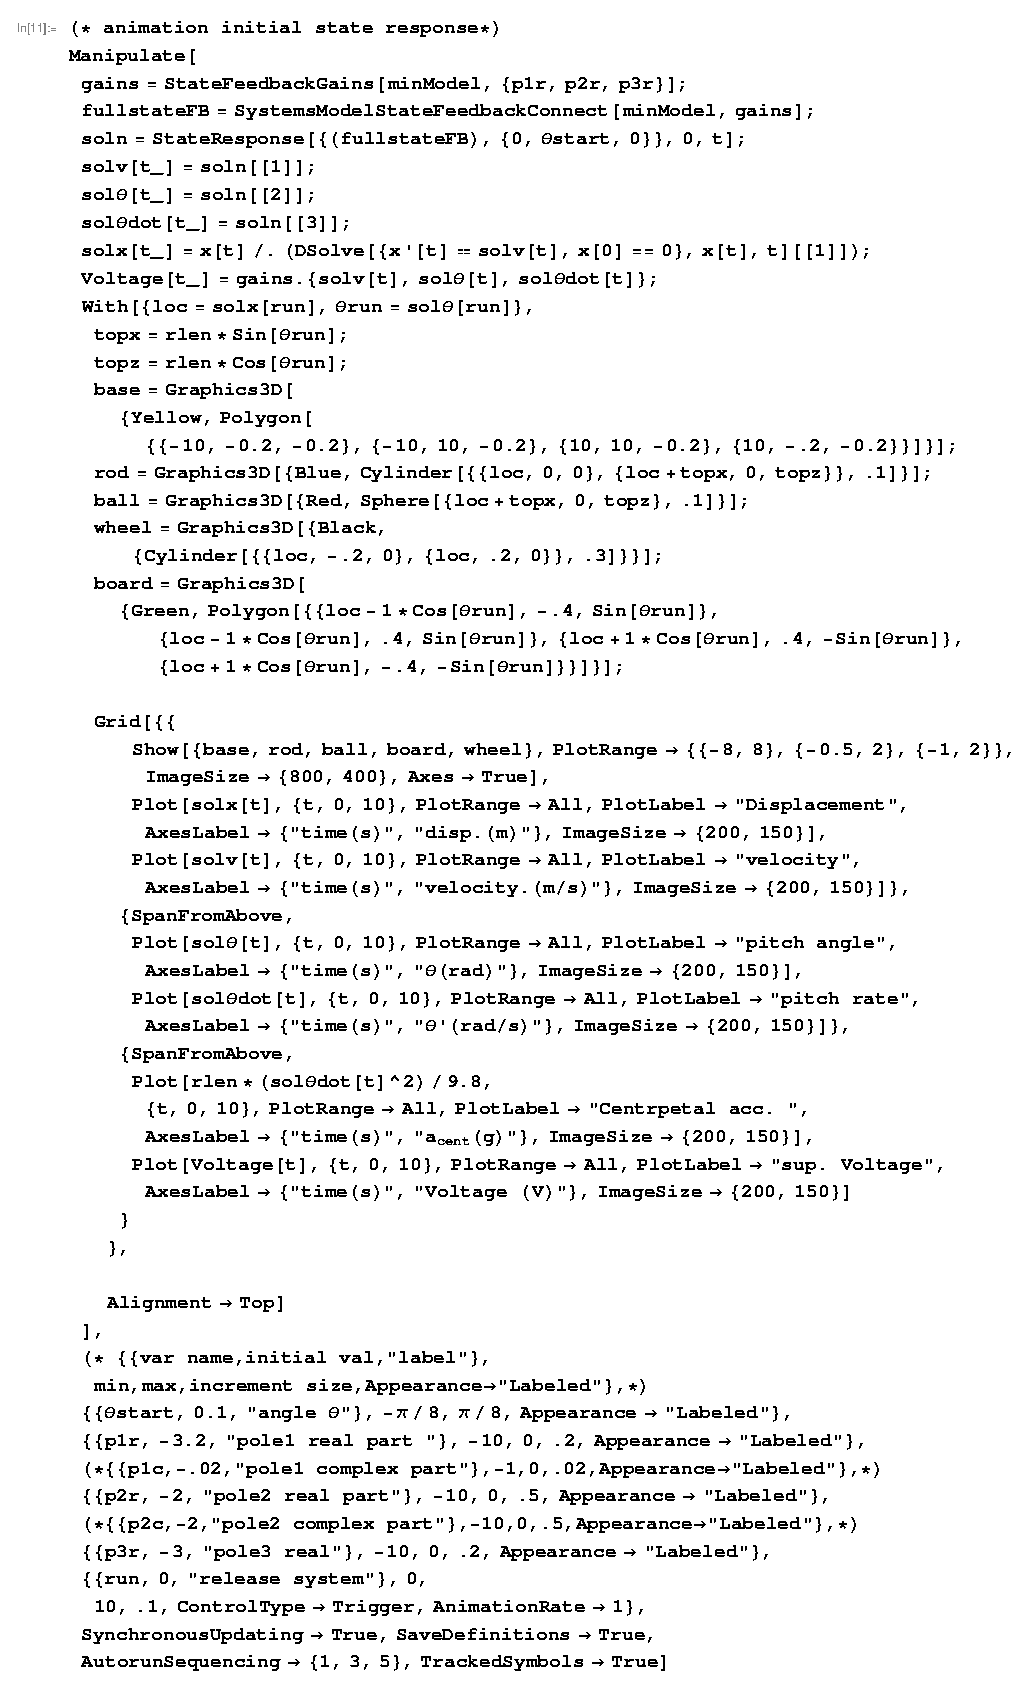
\includegraphics[width=0.6 \linewidth]{code2.eps}
		  \caption{Code added for simulation and visualization}
		  \label{fig:6.2}
	\end{figure}
\newpage
	\begin{figure}[!ht]
			\centering
			  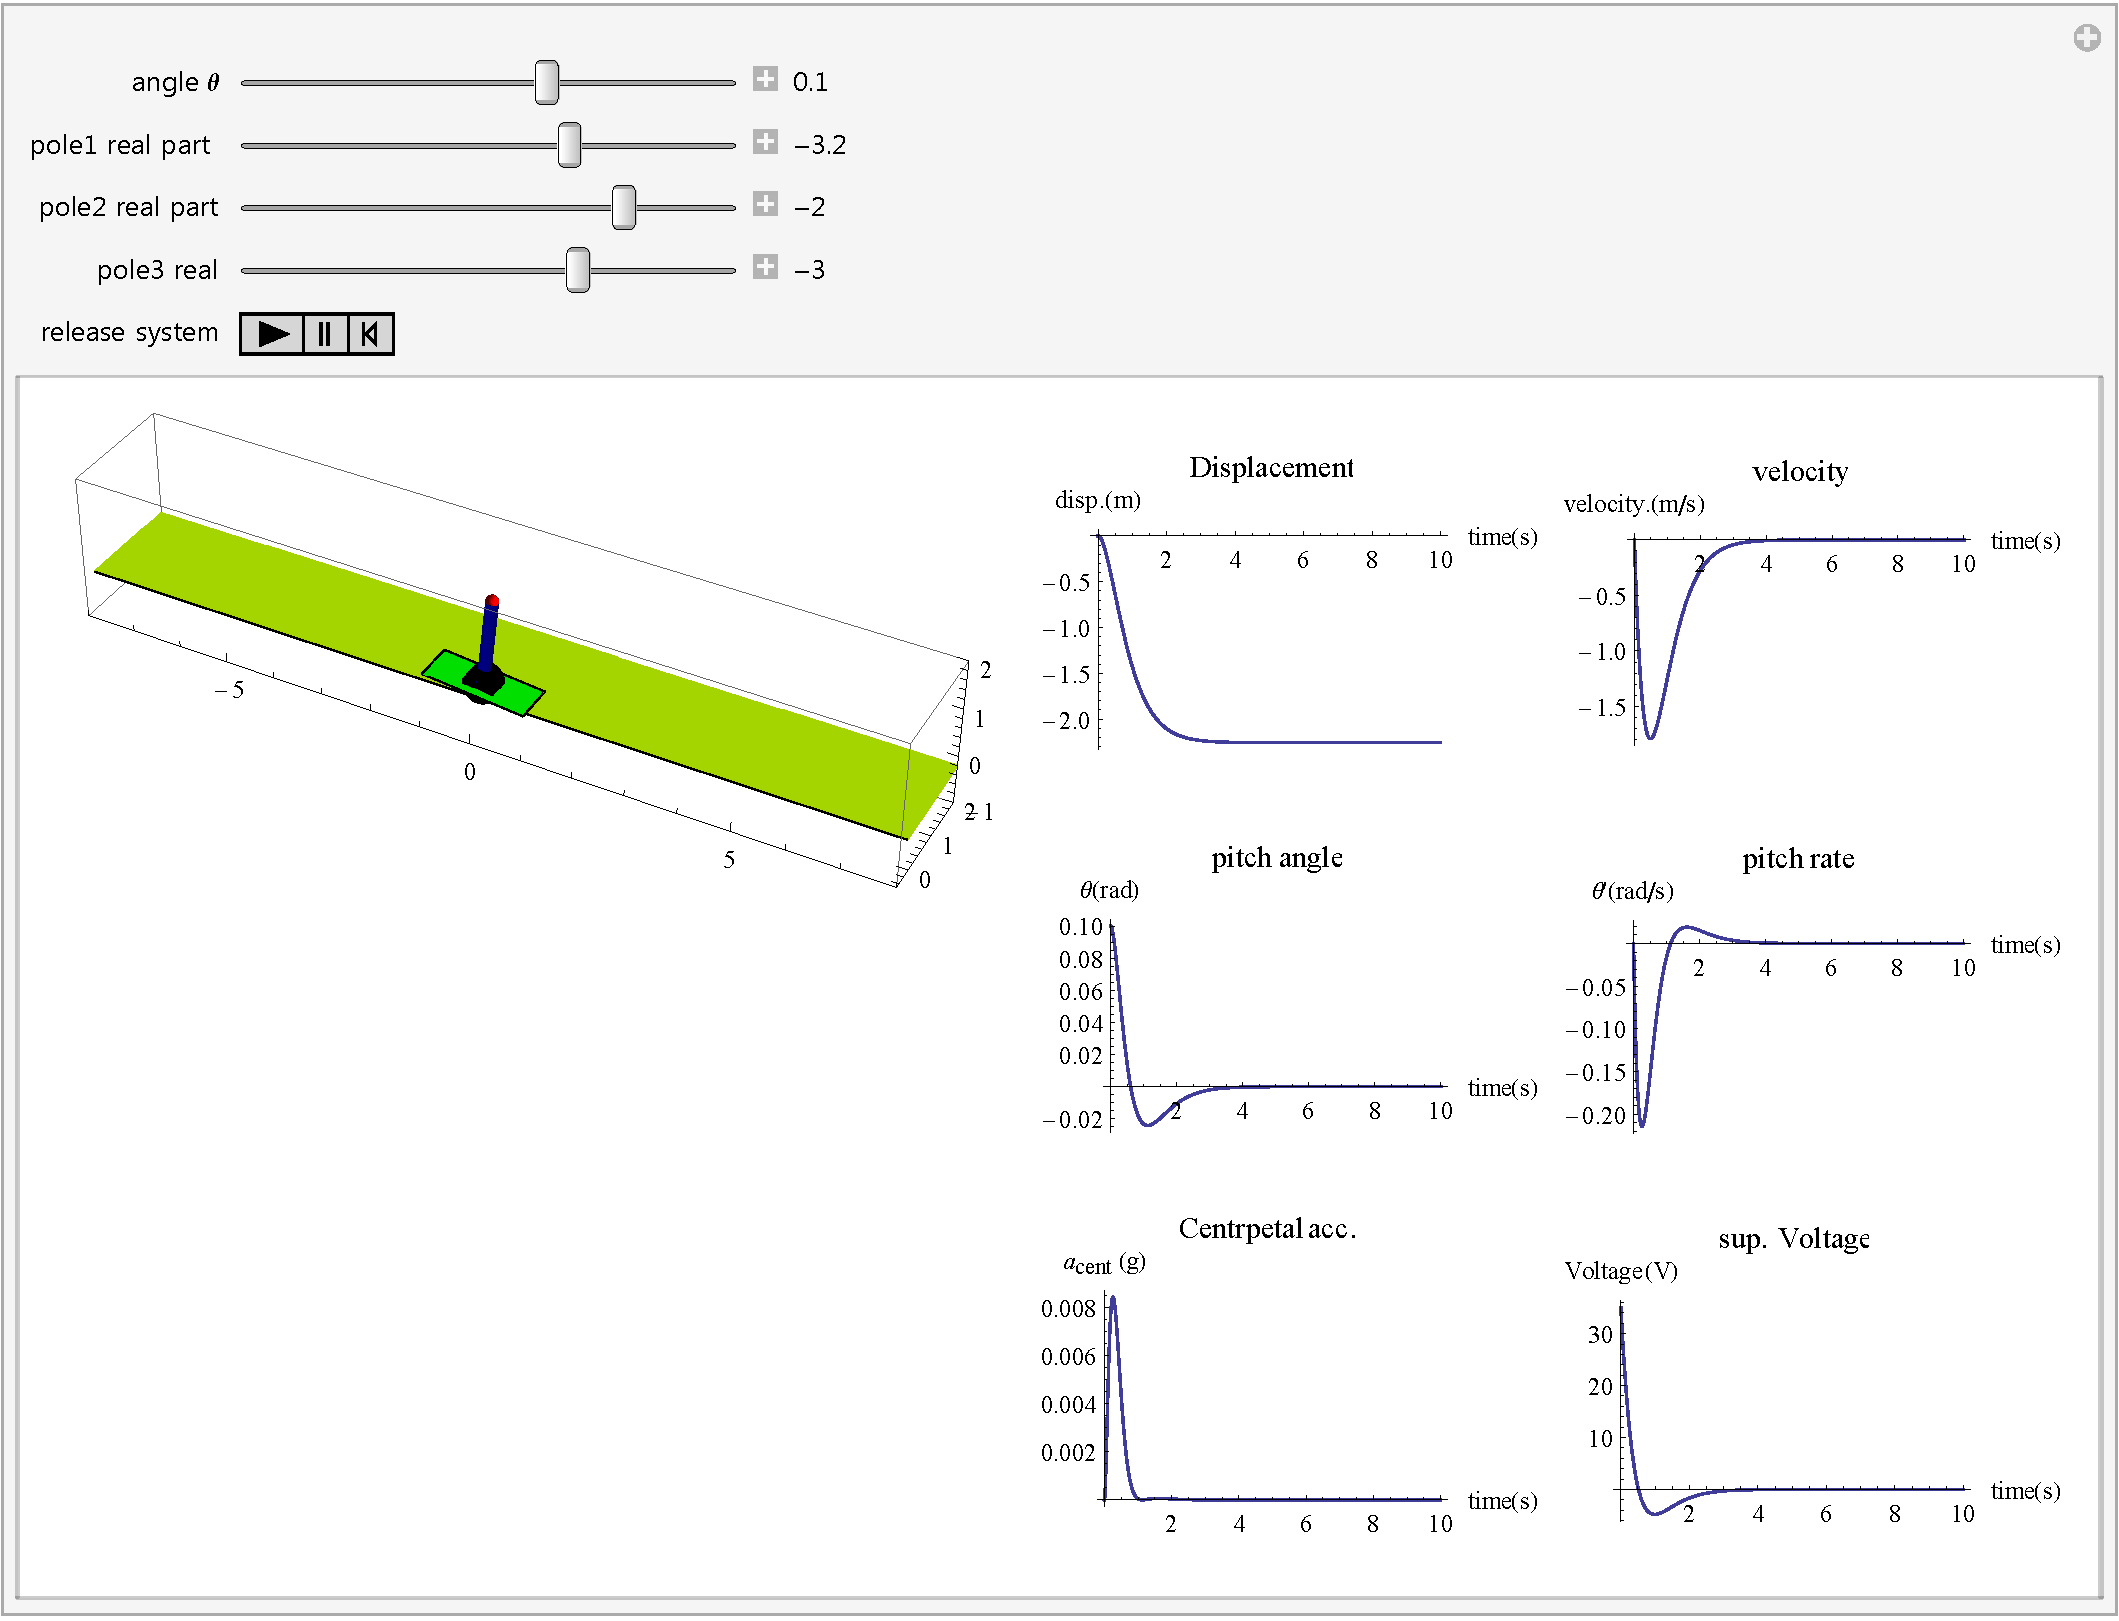
\includegraphics[width=1 \linewidth]{simulation}
			  \caption{Dynamic simulation}
			  \label{fig:6.3}
		\end{figure}
\textbf{Physical parameters of the system}
\begin{table}[h!]
\begin{tabular}{|l|l|l|}
\hline
Mw & Mass of the wheels                                         & 4     \\ \hline
Mb & Mass of the pendulum                                       & 120   \\ \hline
Ke & Motor constant                                             & 0.083 \\ \hline
Km & Motor constant                                             & 0.069 \\ \hline
R  & Motor armature resistance                                  & 1     \\ \hline
Rw & Radius of wheels                                           & 0.2   \\ \hline
L  & Height of the pendulum (person)                            & 1.8   \\ \hline
Jb & Moment of inertia of the person about their center of mass & 60    \\ \hline
Jw & Moment of inertia of wheels                                & 0.07  \\ \hline
g  & Acceleration due to gravity                                & 9.8   \\ \hline
\end{tabular}
\end{table}
\end{enumerate}

\pagebreak
\section{\textit{References}}
\begin{enumerate}
\item Grasser, Felix, et al. "JOE: a mobile, inverted pendulum." Industrial Electronics, IEEE Transactions on 49.1 (2002): 107-114.
\item Thao, Nguyen Gia Minh, Duong Hoai Nghia, and Nguyen Huu Phuc. "A PID backstepping controller for two-wheeled self-balancing robot." Strategic Technology (IFOST), 2010 International Forum on. IEEE, 2010.
\item https://www.sparkfun.com/products/10736
\item https://www.sparkfun.com/products/9873        
\item http://arduino.cc/en/Main/ArduinoBoardUno
 
\end{enumerate}
\end{document}
